\section{Introduction}
Here we analysed the functional connectivity of the brain using 6-channel EEG data for four different states: eyes open, eyes closed, while concentrating and while meditating. For this data we computed 
comparison of connectivity window vectors used KMeans clustering to classify brain states and plotted circular plots showing relations between brain regions.









\section{Open eyes}


\begin{figure}[h!]
\begin{minipage}[h]{0.49\linewidth}
\center{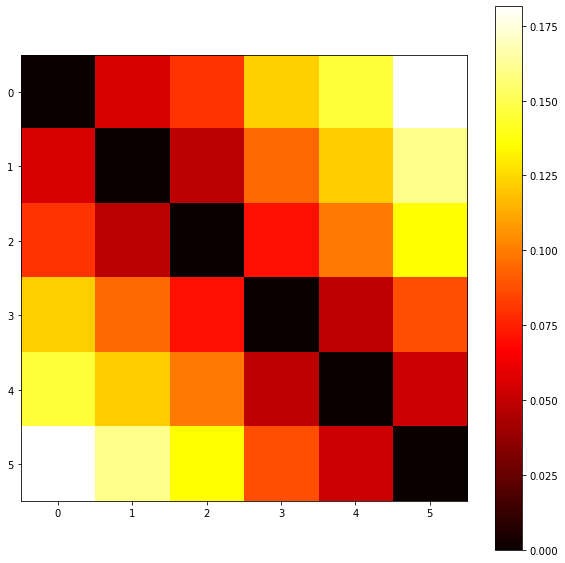
\includegraphics[width=0.9\linewidth]{sections/R_O_heatmap.png}} (a) \\
\end{minipage}
\hfill
\begin{minipage}[h]{0.5\linewidth}
\center{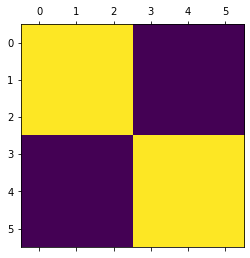
\includegraphics[width=0.9\linewidth]{sections/R_O_heatmap_clusters.png}} (b) \\
\end{minipage}
\caption{Comparison of connectivity window vectors with open eyes: a) full b) simplified clusters} 
\end{figure}

\begin{figure}[h!]
\begin{minipage}[h]{0.49\linewidth}
\center{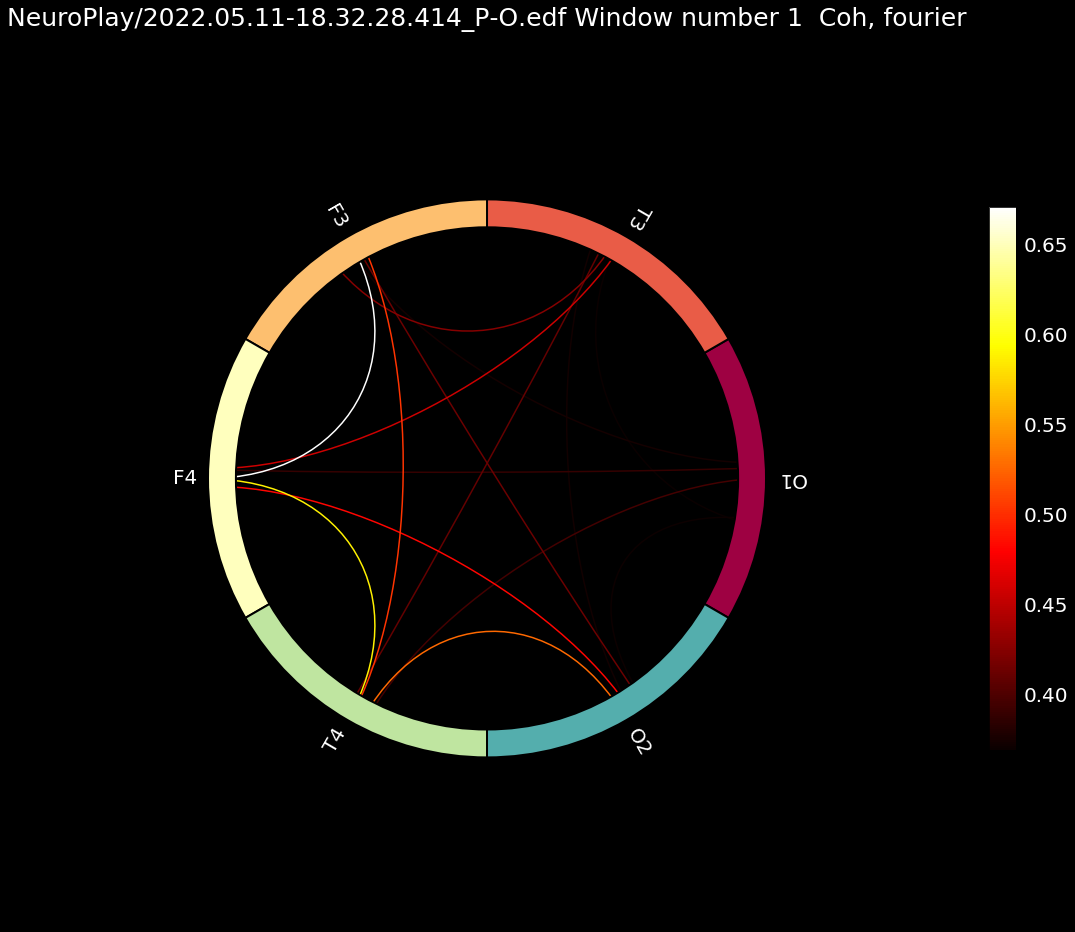
\includegraphics[width=0.9\linewidth]{sections/R_O_circle.png}} (a) \\
\end{minipage}
\hfill
\begin{minipage}[h]{0.5\linewidth}
\center{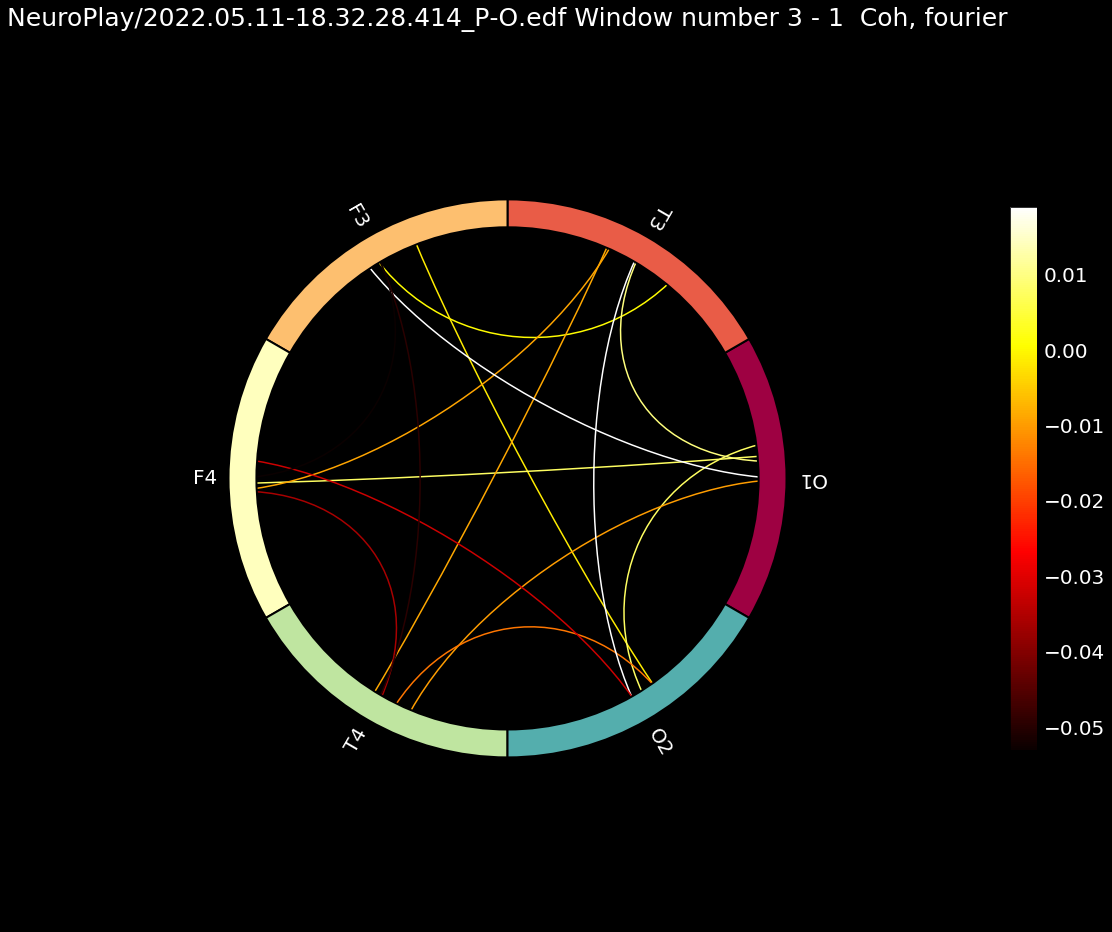
\includegraphics[width=0.9\linewidth]{sections/R_O_circle_delta.png}} (b) \\
\end{minipage}
\caption{Connectivity with open eyes: a) ordinary b) time shift} 
\end{figure}
\par Here we can see that state is changing dramatically during the process of measurement, clustering suggests that there was two different states in the beginning and in the end.
\par As for circular plot, we can see that Signals from F3 and F4 are most coherent, and the plot with time shift represents dramatic changes in the state during measurement.


\vspace*{2cm}


\section{Closed eyes}

\par Heatmap clearly shows that with closed eyes brain remains in only one state and K means clustering confirms that.
\par Circular plot shows strong connection between F4 and T4 electrodes

\begin{figure}[h!]
\begin{minipage}[h]{0.49\linewidth}
\center{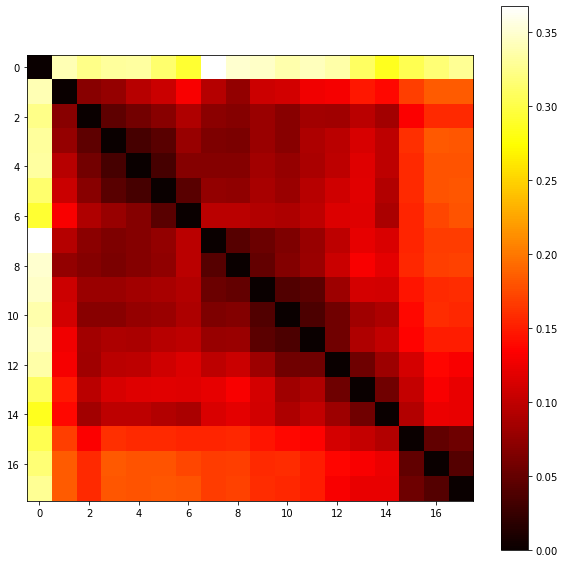
\includegraphics[width=1\linewidth]{sections/R_Z_heatmap.png}} (a) \\
\end{minipage}
\hfill
\begin{minipage}[h]{0.5\linewidth}
\center{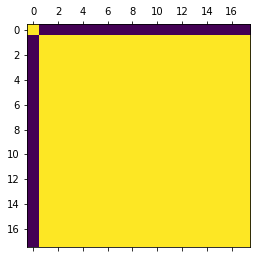
\includegraphics[width=1\linewidth]{sections/R_Z_heatmap_clusters.png}} (b) \\
\end{minipage}
\caption{Comparison of connectivity window vectors with closed eyes: a) full b) simplified clusters} 
\end{figure}

\begin{figure}[h!]
\begin{minipage}[h]{0.49\linewidth}
\center{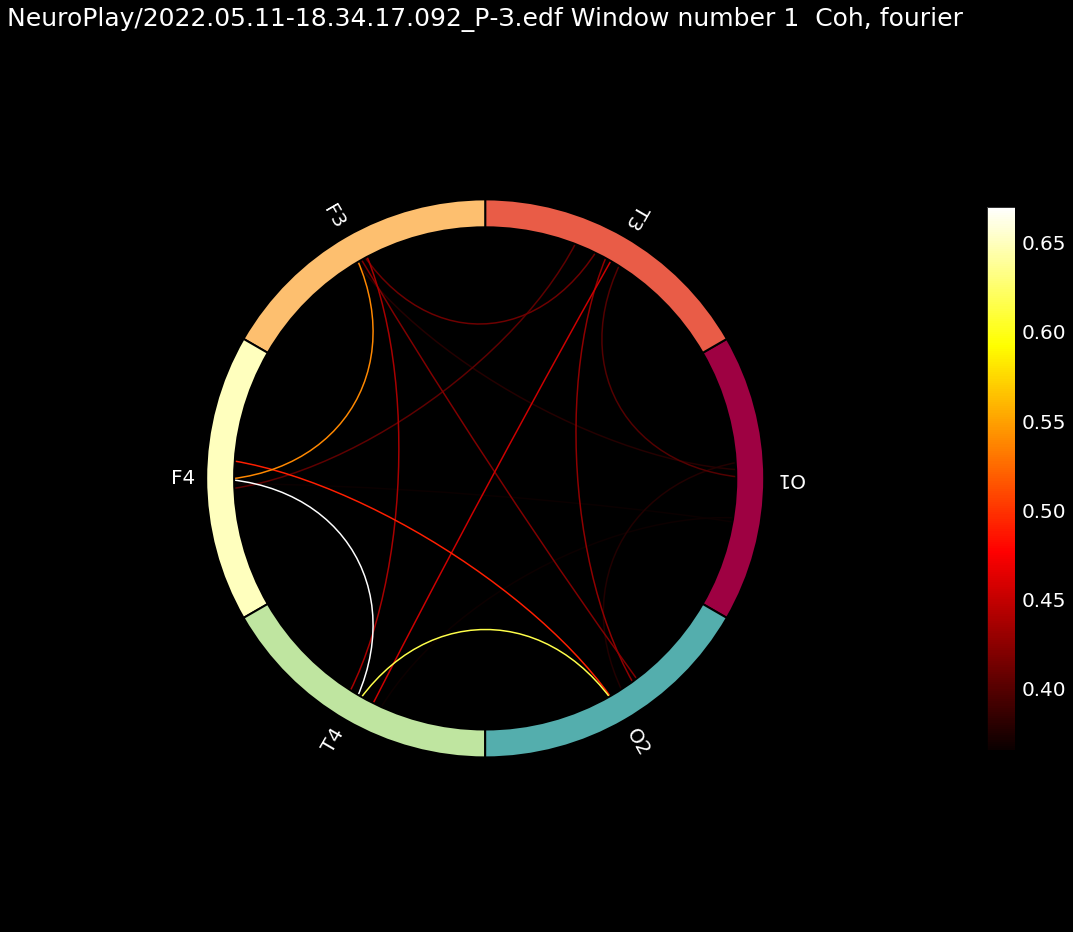
\includegraphics[width=1\linewidth]{sections/R_Z_circle.png}} (a) \\
\end{minipage}
\hfill
\begin{minipage}[h]{0.5\linewidth}
\center{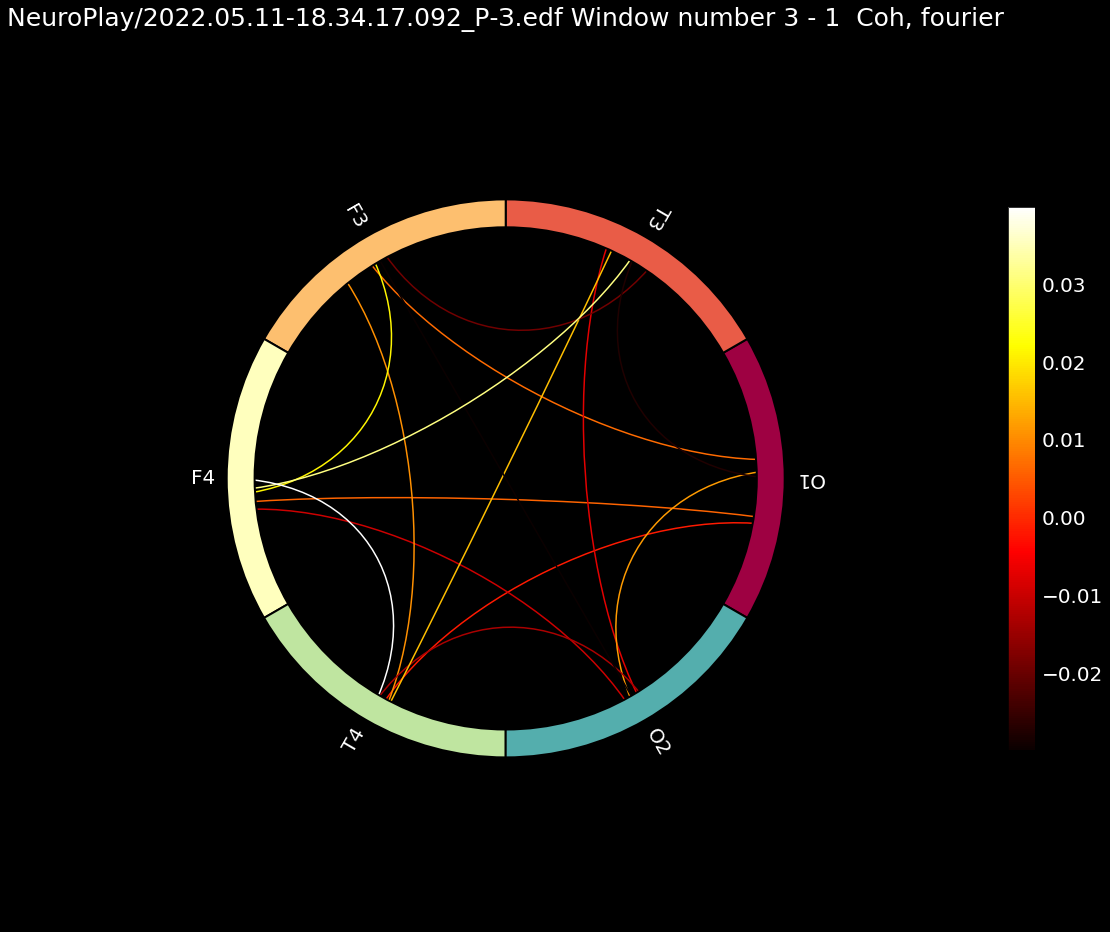
\includegraphics[width=1\linewidth]{sections/R_Z_circle_delta.png}} (b) \\
\end{minipage}
\caption{Connectivity with closed eyes: a) ordinary b) time shift} 
\end{figure}




\vspace*{4cm}







\section{Concentration}
\par Comparison of connectivity window vectors shows two independent states, first of which was interrupted for a short period of time.
\par Again we have strong connection between F3 and F4, but we also can see distant coherence between F and O electrodes, which show up in brains of creative people.[1] 

\begin{figure}[h!]
\begin{minipage}[h]{0.49\linewidth}
\center{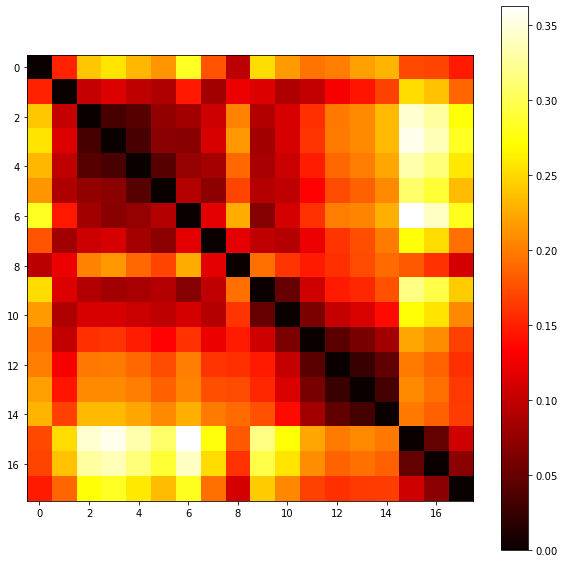
\includegraphics[width=1\linewidth]{sections/R_K_heatmap.png}} (a) \\
\end{minipage}
\hfill
\begin{minipage}[h]{0.5\linewidth}
\center{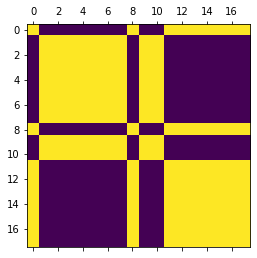
\includegraphics[width=1\linewidth]{sections/R_K_heatmap_clusters.png}} (b) \\
\end{minipage}
\caption{Comparison of connectivity window vectors for concentration training: a) full b) simplified clusters} 
\end{figure}

\begin{figure}[h!]
\begin{minipage}[h]{0.49\linewidth}
\center{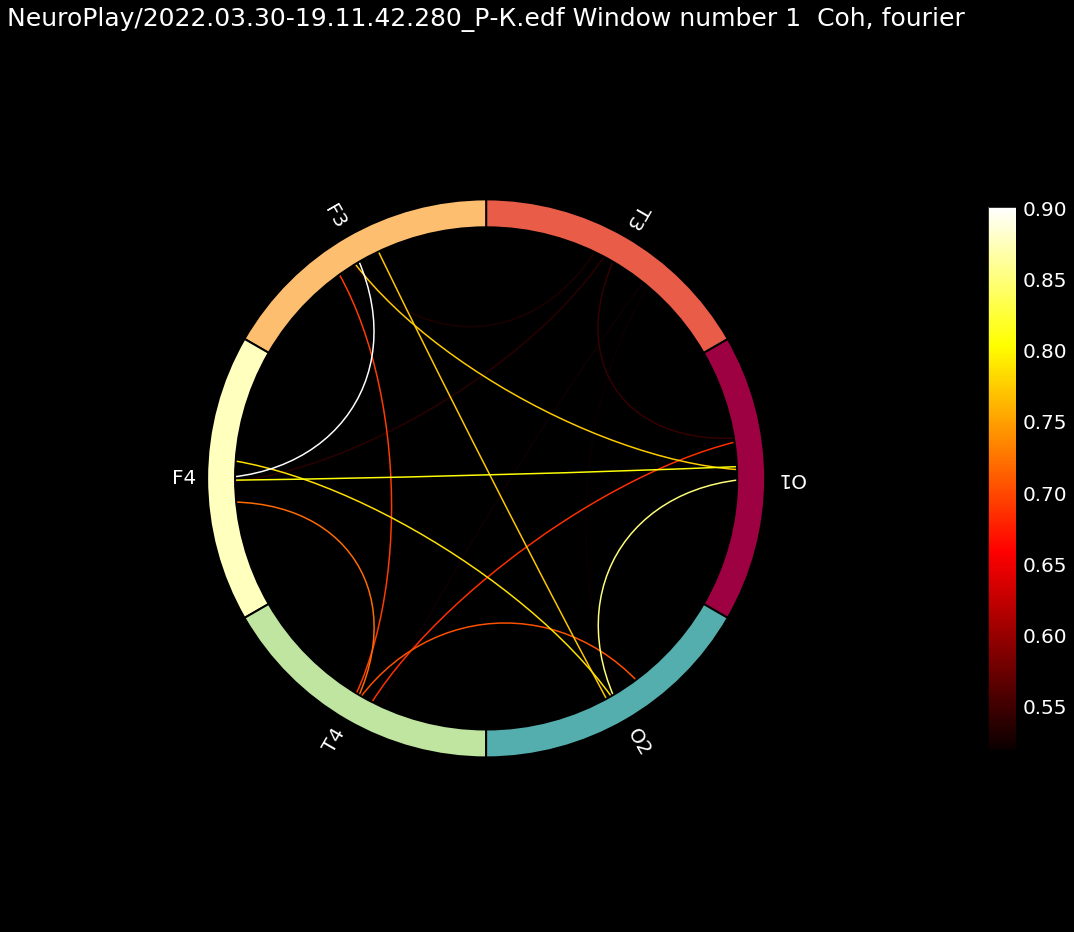
\includegraphics[width=1\linewidth]{sections/R_K_circle.png}} (a) \\
\end{minipage}
\hfill
\begin{minipage}[h]{0.5\linewidth}
\center{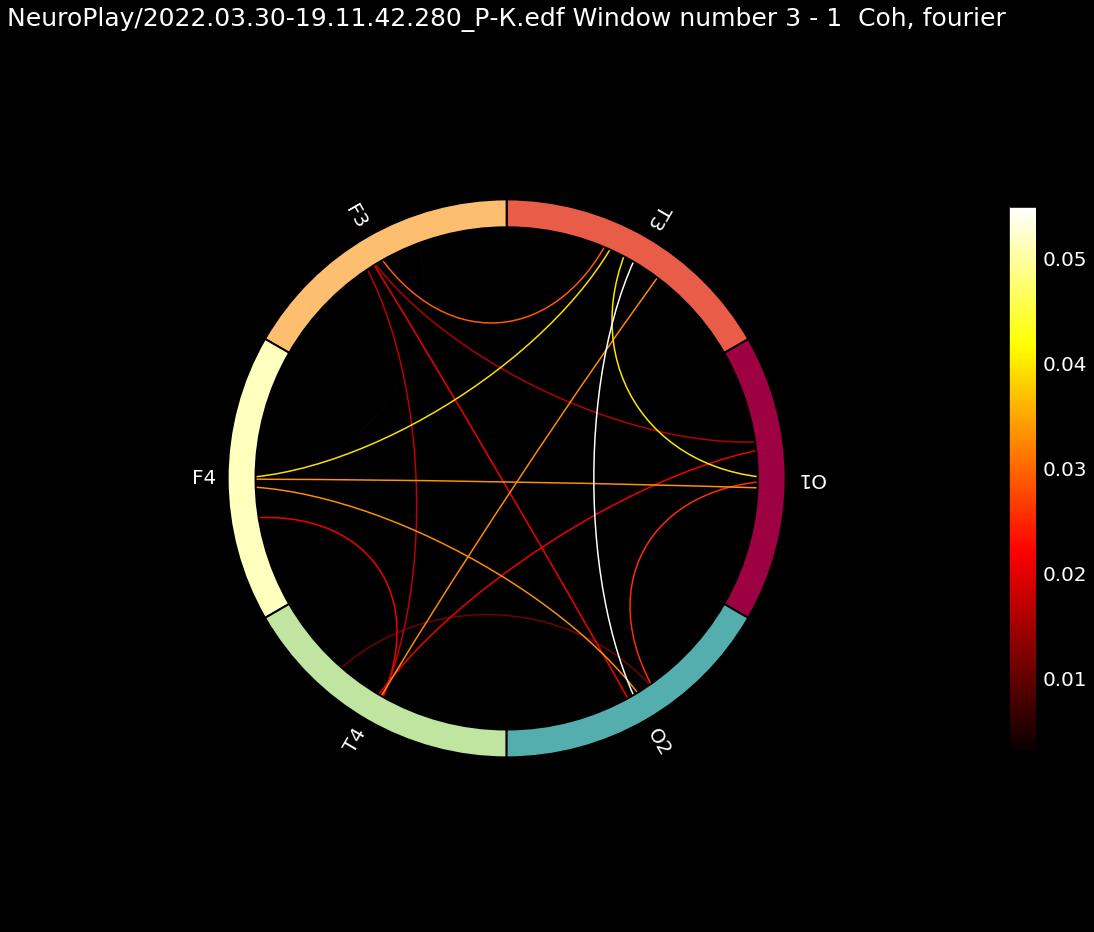
\includegraphics[width=1\linewidth]{sections/R_K_circle_delta.png}} (b) \\
\end{minipage}
\caption{Connectivity for concentration training: a) ordinary b) time shift} 
\end{figure}


\vspace*{2cm}


\section{Meditation}
\par There we can see that the first state was interrupted by the second state, and then the first state repeats.
\par picture on the circular plot is the same as for concentration except the connection between F and O electrodes is much weaker.

\begin{figure}[h!]
\begin{minipage}[h]{0.49\linewidth}
\center{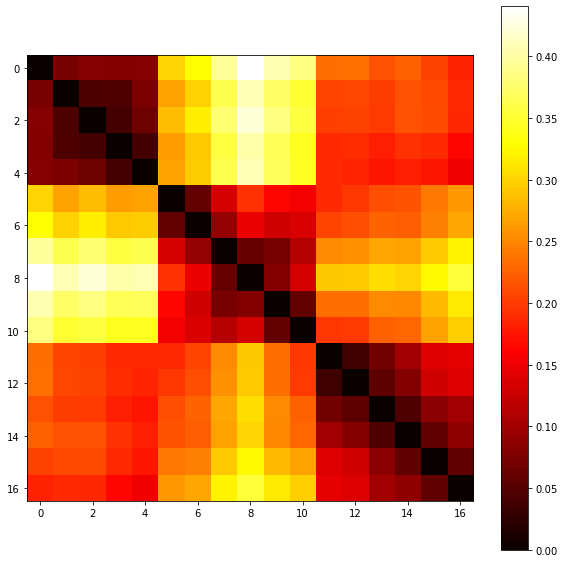
\includegraphics[width=1\linewidth]{sections/R_M_heatmap.png}} (a) \\
\end{minipage}
\hfill
\begin{minipage}[h]{0.5\linewidth}
\center{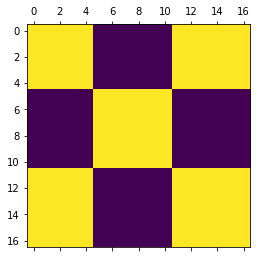
\includegraphics[width=1\linewidth]{sections/R_M_heatmap_clusters.png}} (b) \\
\end{minipage}
\caption{Comparison of connectivity window vectors for meditation training: a) full b) simplified clusters} 
\end{figure}


\begin{figure}[h!]
\begin{minipage}[h]{0.49\linewidth}
\center{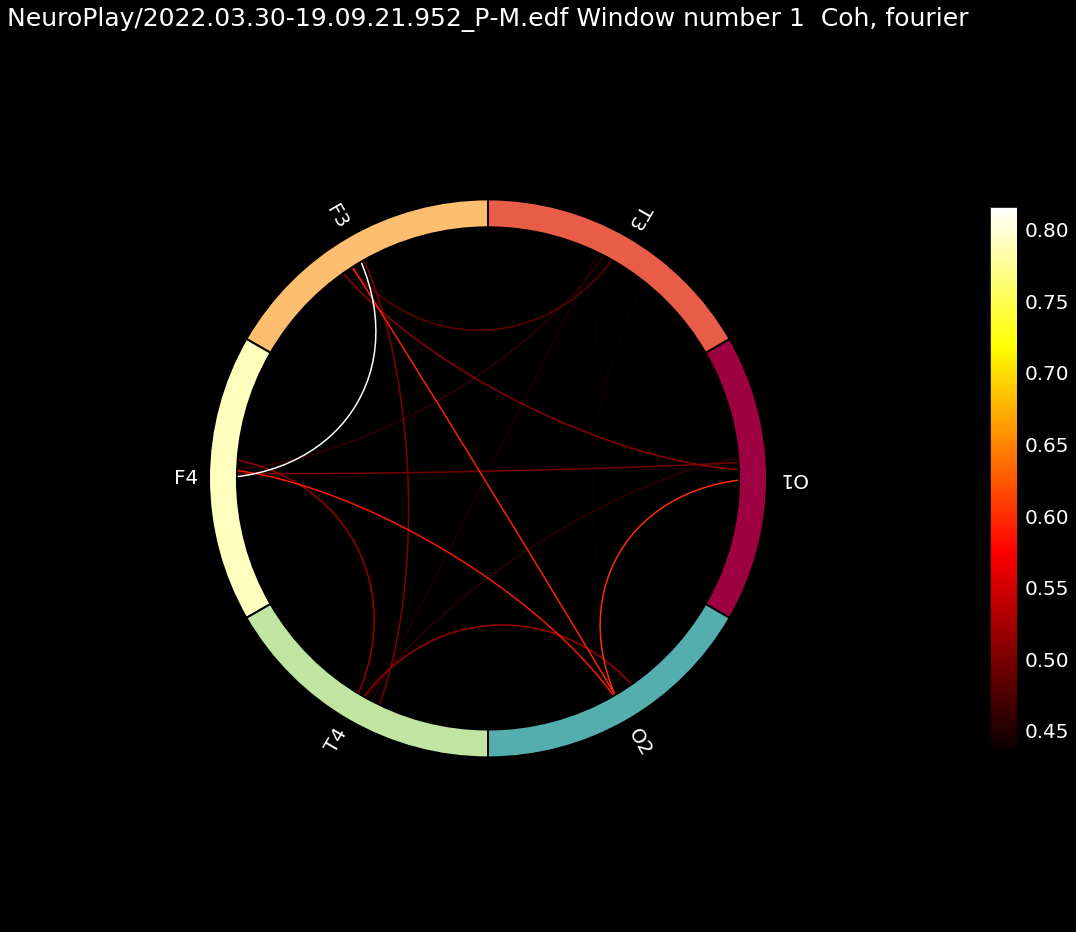
\includegraphics[width=1\linewidth]{sections/R_M_circle.png}} (a) \\
\end{minipage}
\hfill
\begin{minipage}[h]{0.5\linewidth}
\center{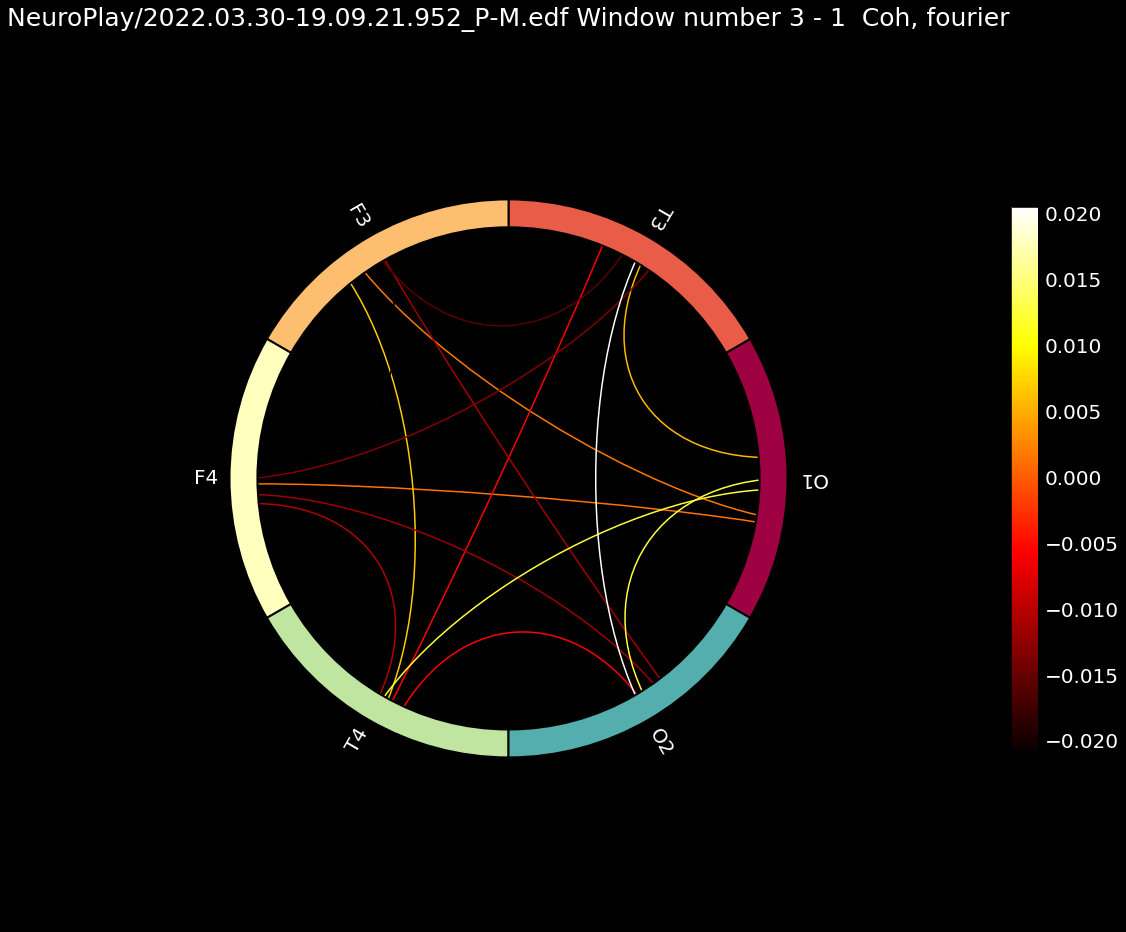
\includegraphics[width=1\linewidth]{sections/R_M_circle_delta.png}} (b) \\
\end{minipage}
\caption{Connectivity for meditation training: a) ordinary b) time shift} 
\end{figure}

\vspace*{4cm}

\section{Functional connectivity difference}
\par There is a considerable difference between states with open/closed eyes in the way F3 and F4 are connected. Those electrodes were located in the visual cortex which explains why connectivity between F3 and F4 was the highest when the subject had their eyes open. It shows that the brain was comparing and contrasting information from both eyes.

\begin{figure}[h!]
\begin{minipage}[h]{0.49\linewidth}
\center{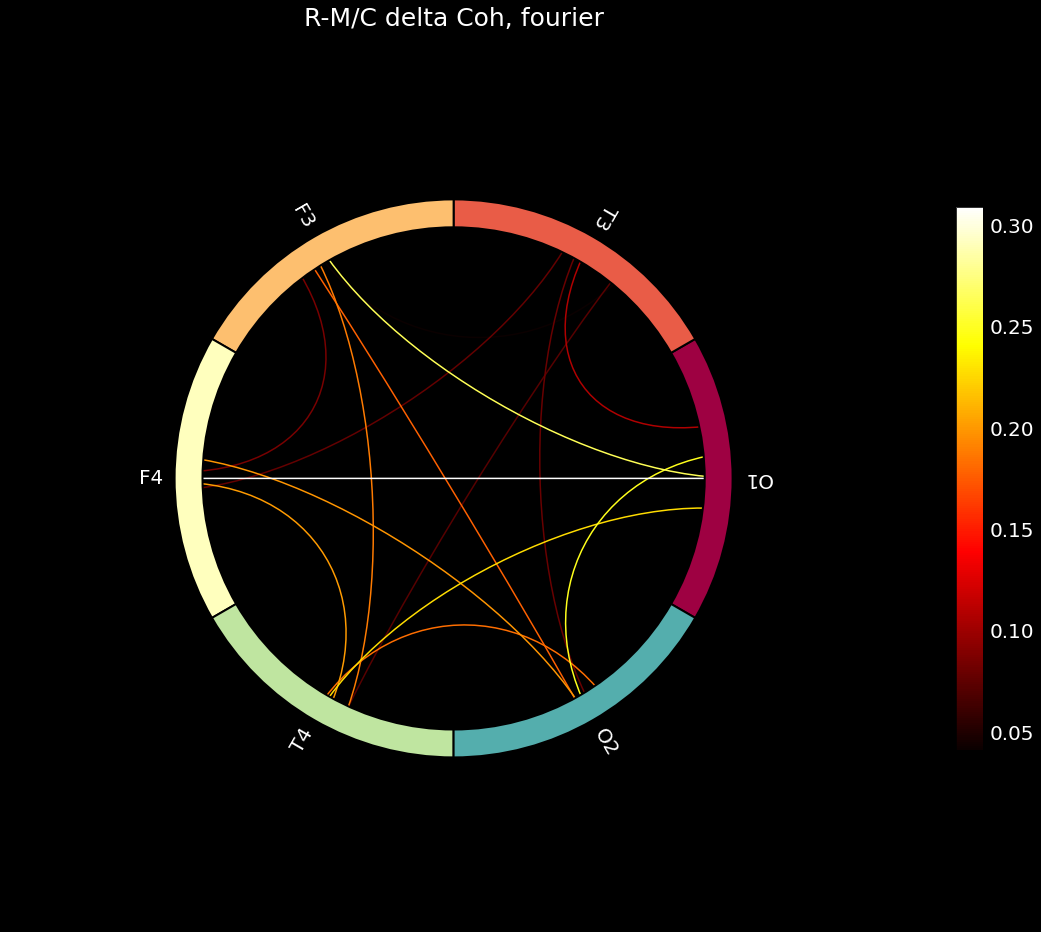
\includegraphics[width=0.7\linewidth]{sections/difference_concentration_meditation.png}} (a) \\
\end{minipage}
\hfill
\begin{minipage}[h]{0.5\linewidth}
\center{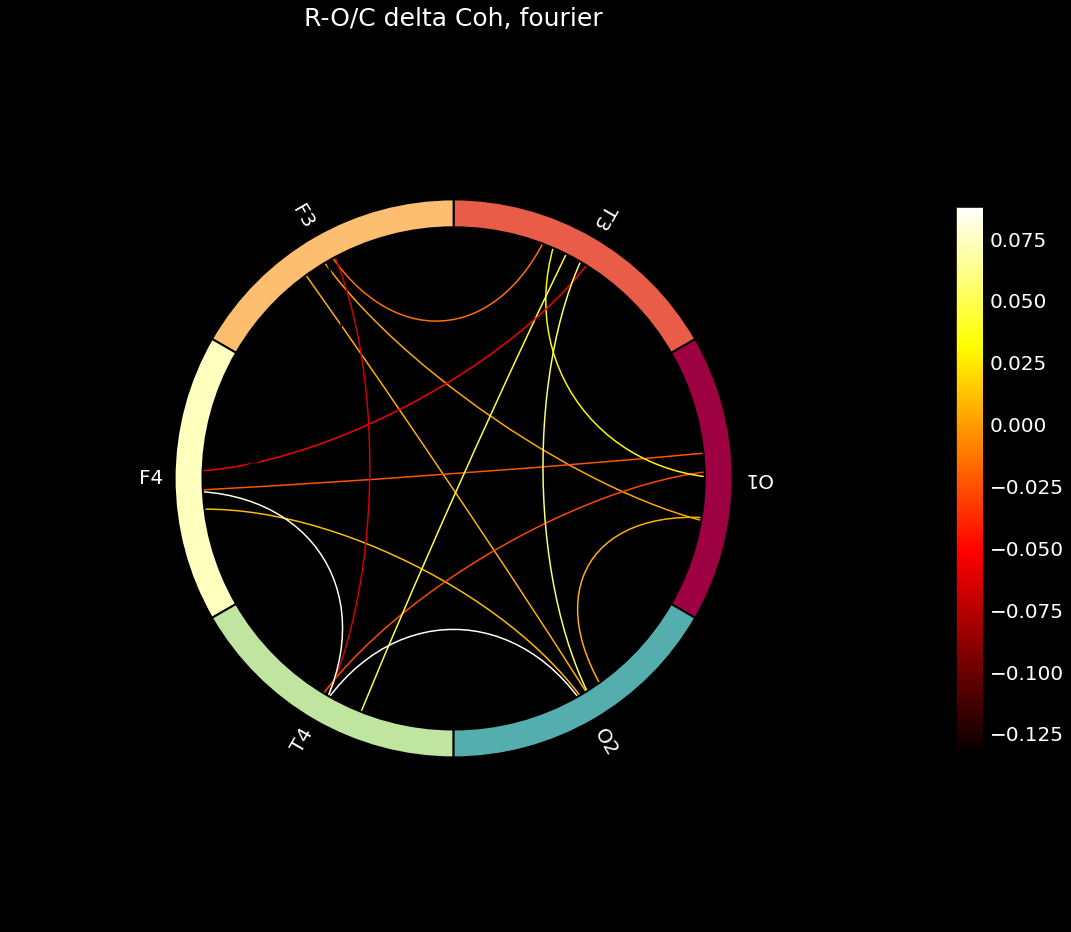
\includegraphics[width=0.7\linewidth]{sections/difference_open_closed.png}} (b) \\
\end{minipage}
\caption{a) Difference between concentration and meditation training b) Difference between open and closed eyes} 
\end{figure}


\begin{figure}[h!]
\centering
\fbox{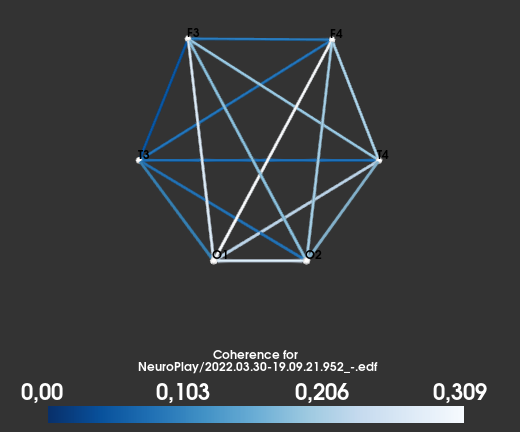
\includegraphics[width=0.35\linewidth]{sections/coherence.png}}
\caption{Coherence}
\end{figure}


\par It can be concluded that concentration training was aimed to strengthen the frontoparietal connectivity. Meditation training seemed to comparatively increase connectivity between T and O electrodes, which could be a sign of increased connectivity between attentional regions and medial frontal regions as per [2]. The effects of meditation cannot be concluded for certain because the reference study compared experienced and not experienced meditators and our subject was not experienced









\section{Rhythms}

We are going to be comparing the whole picture from concentration with the different bands. The goal is to determine if there is any major information in the different frequency bands that gets lost in the whole picture.


\begin{figure}[h!]
\begin{minipage}[h]{0.49\linewidth}
\center{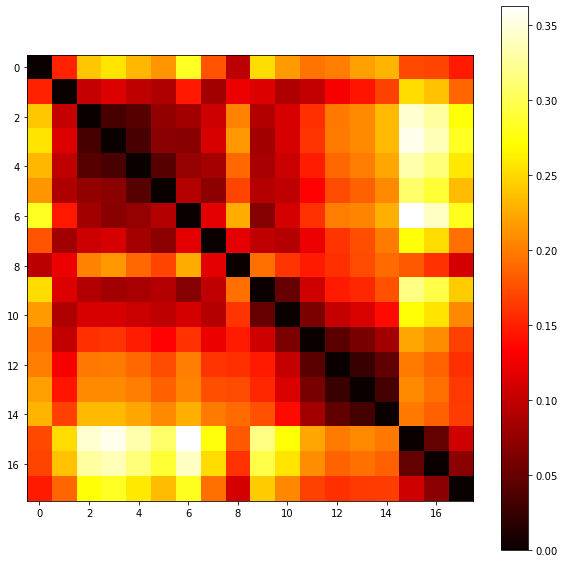
\includegraphics[width=1\linewidth]{sections/R_K_heatmap.png}} (a) \\
\end{minipage}
\hfill
\begin{minipage}[h]{0.5\linewidth}
\center{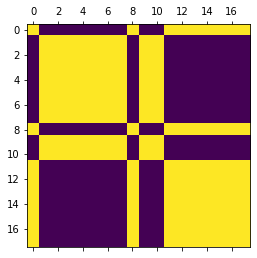
\includegraphics[width=1\linewidth]{sections/R_K_heatmap_clusters.png}} (b) \\
\end{minipage}
\caption{All frequency bands} 
\end{figure}

\begin{figure}[h!]
\begin{minipage}[h]{0.49\linewidth}
\center{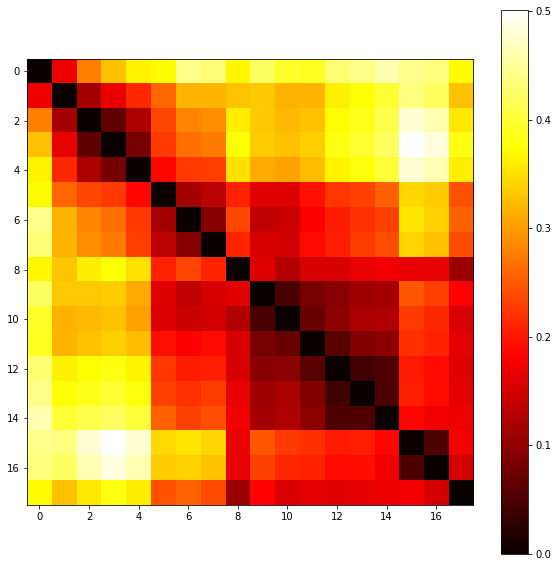
\includegraphics[width=1\linewidth]{sections/alpha_heatmap.png}} (a) \\
\end{minipage}
\hfill
\begin{minipage}[h]{0.5\linewidth}
\center{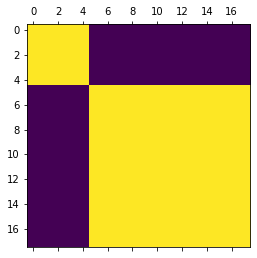
\includegraphics[width=1\linewidth]{sections/alpha_heatmap_clusters.png}} (b) \\
\end{minipage}
\caption{Only alpha frequency band} 
\end{figure}

\begin{figure}[h!]
\begin{minipage}[h]{0.49\linewidth}
\center{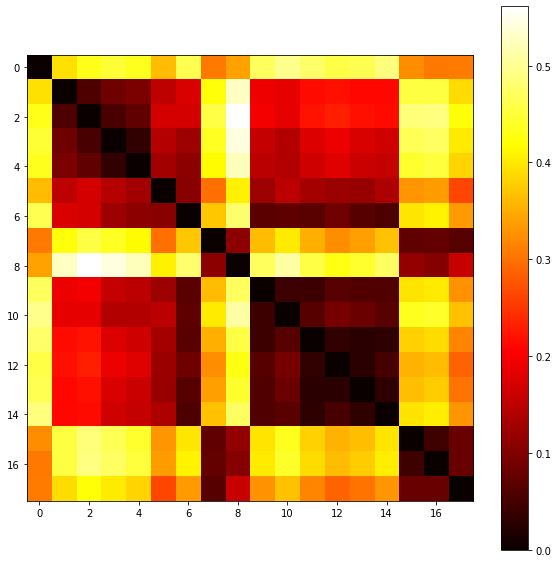
\includegraphics[width=1\linewidth]{sections/beta1_heatmap.png}} (a) \\
\end{minipage}
\hfill
\begin{minipage}[h]{0.5\linewidth}
\center{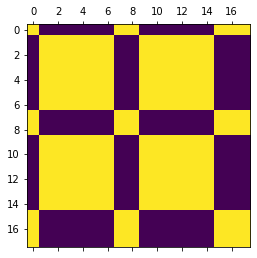
\includegraphics[width=1\linewidth]{sections/beta1_heatmap_clusters.png}} (b) \\
\end{minipage}
\caption{Only beta-1 frequency band} 
\end{figure}

\begin{figure}[h!]
\begin{minipage}[h]{0.49\linewidth}
\center{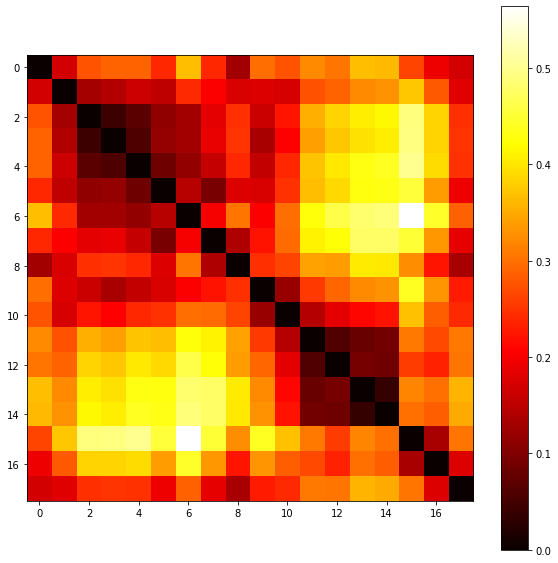
\includegraphics[width=1\linewidth]{sections/beta2_heatmap.png}} (a) \\
\end{minipage}
\hfill
\begin{minipage}[h]{0.5\linewidth}
\center{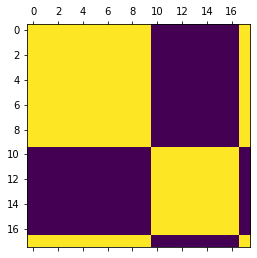
\includegraphics[width=1\linewidth]{sections/beta2_heatmap_clusters.png}} (b) \\
\end{minipage}
\caption{Only beta-2 frequency band} 
\end{figure}

\begin{figure}[h!]
\begin{minipage}[h]{0.49\linewidth}
\center{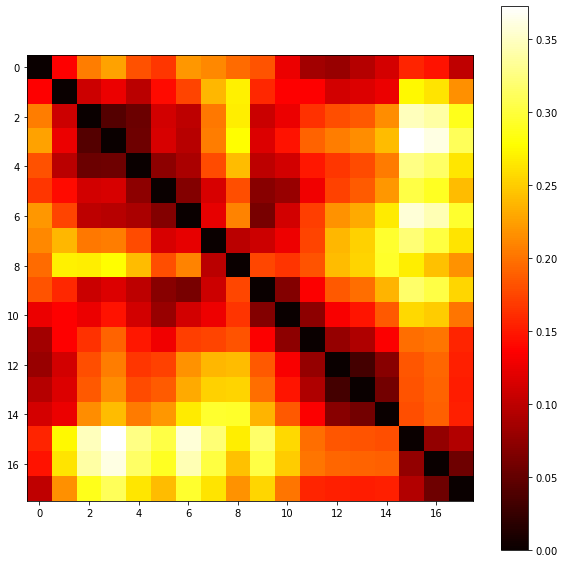
\includegraphics[width=1\linewidth]{sections/gamma_heatmap.png}} (a) \\
\end{minipage}
\hfill
\begin{minipage}[h]{0.5\linewidth}
\center{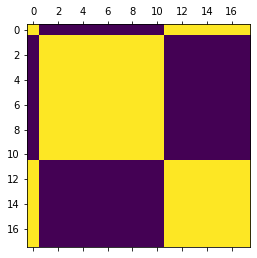
\includegraphics[width=1\linewidth]{sections/gamma_heatmap_clusters.png}} (b) \\
\end{minipage}
\caption{Only gamma frequency band} 
\end{figure}

\begin{figure}[h!]
\begin{minipage}[h]{0.49\linewidth}
\center{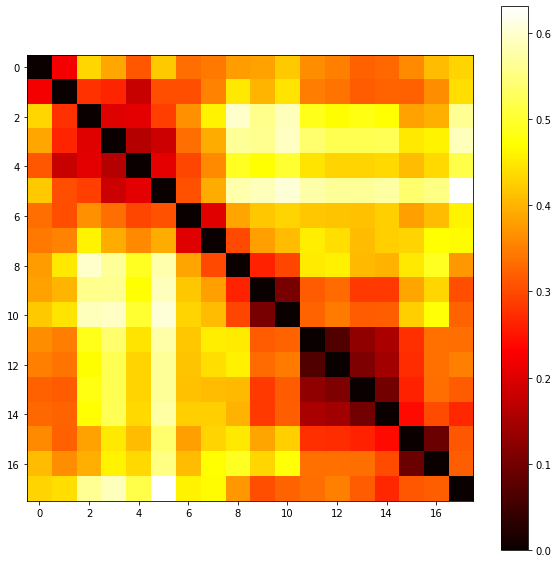
\includegraphics[width=1\linewidth]{sections/delta_heatmap.png}} (a) \\
\end{minipage}
\hfill
\begin{minipage}[h]{0.5\linewidth}
\center{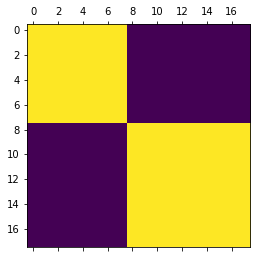
\includegraphics[width=1\linewidth]{sections/delta_heatmap_clusters.png}} (b) \\
\end{minipage}
\caption{Only delta frequency band} 
\end{figure}

\begin{figure}[h!]
\begin{minipage}[h]{0.49\linewidth}
\center{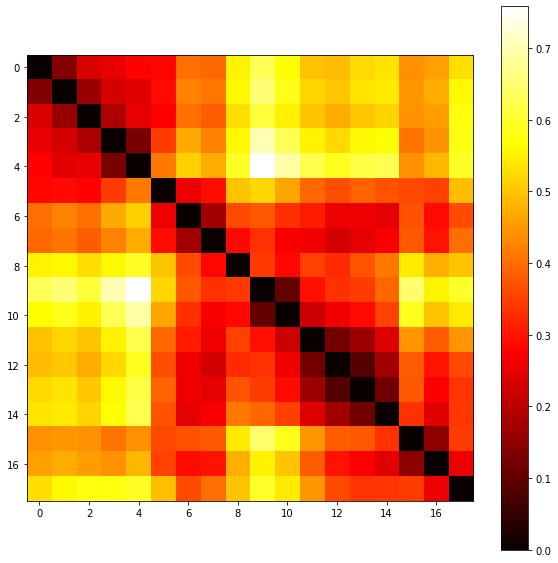
\includegraphics[width=1\linewidth]{sections/theta_heatmap.png}} (a) \\
\end{minipage}
\hfill
\begin{minipage}[h]{0.5\linewidth}
\center{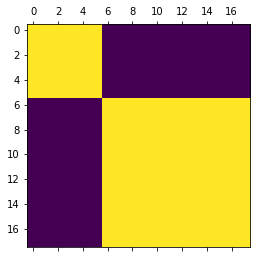
\includegraphics[width=1\linewidth]{sections/theta_heatmap_clusters.png}} (b) \\
\end{minipage}
\caption{Only theta frequency band} 
\end{figure}

\par As mentioned above, there are two different states observed during concentration training. After the spectral decomposition of the signal, we can conclude that waves of almost all frequencies changed, only beta-1 waves fluctuated around one state. 
\par Also from the fact that the whole state switched at the exact time gamma frequency waves changed, we can suppose that it was a trigger factor for state switching. Gamma brain waves are associated with high levels of thought and focus[https://www.webmd.com/brain/what-to-know-about-gamma-brain-waves] so it is unsurprising that gamma waves were main waves in the state of concentration.
\par We can say that difference between specific frequency bands and overall information depends dramatically on the observed state.



 
